% !TEX root = ../../prj4projektdokumentation.tex

\subsection{Kalibrering af måleenhed.}

Efter test af funktionaliteten af Måleenheden laves en kalibrering, for at fjerne det offset, som er opstået i forbindelse med forstærkning/dæmpning af signal i hardwaren. 

\subsubsection{Måleopstilling}

Til kalibrering af måleenheden er anvendes en funktionsgenerator, til at lave sinussignalet, som forbindes direkte til måleenheden. Til korrekt måling af spændingsværdier anvendes oscilloskop, som her antages for værende ideel. Måleenheden er tilsluttet en PC og kører i debug-mode, så værdierne for strøm og spænding kan aflæses. 
\begin{figure}[H]
	\centering
	\begin{minipage}[b]{0.48\textwidth}
		\centering
		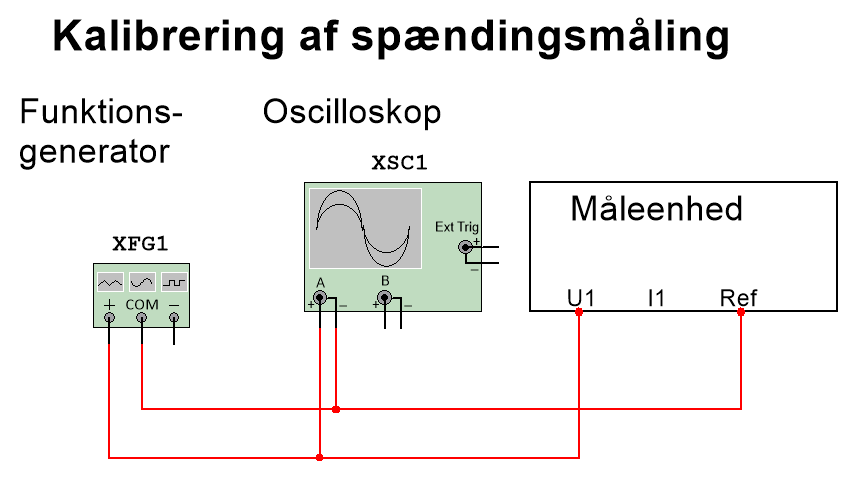
\includegraphics[width=1.00\textwidth]{Figure/MEkalibreringU} % Venstre billede
	\end{minipage}
	\hfill
	\begin{minipage}[b]{0.48\textwidth}
		\centering
		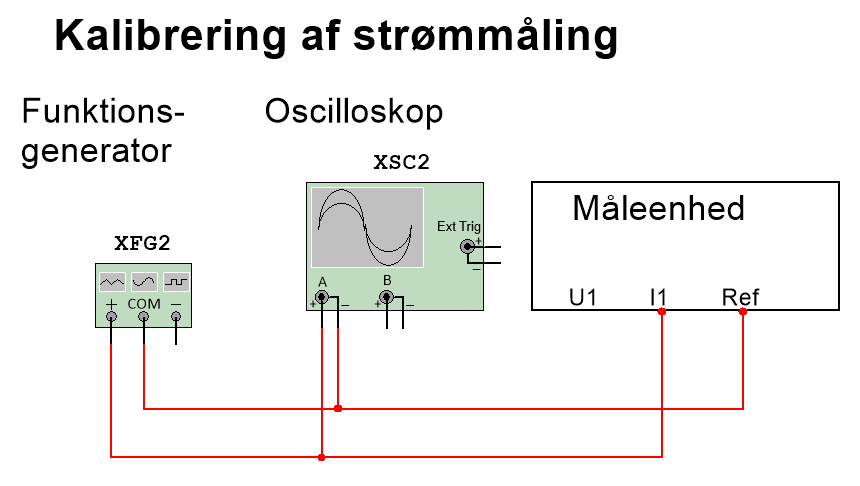
\includegraphics[width=1.00\textwidth]{Figure/MEkalibreringI} % Højre billede
	\end{minipage}
	\\ % Figurtekster og labels
	\begin{minipage}[t]{0.48\textwidth}
		\caption{Måleopstilling for kalibrering af spændingsmåling} % Venstre figurtekst og label
		\label{fig:MEkalibreringU}
	\end{minipage}
	\hfill
	\begin{minipage}[t]{0.48\textwidth}
		\caption{Måleopstilling for kalibrering af strømmåling} % Højre figurtekst og label
		\label{fig:MEkalibreringI}
	\end{minipage}
\end{figure}

\subsubsection{Fremgangsmåde}

Der laves to måleserier, for henholdsvis spænding- og strømmåling. Strømmålingen er baseret på en spændingsmåling over en $1\Omega$ modstand, hvilket betyder at spændingsfaldet over modstanden lig med strømmen. Derfor kalibreres strømmålingen med et spændingssignal, på samme måde som spændingsmålingen. Måleenheden er lavet til at måle en spænding mellem 0-8Vrms og en strøm mellem $\SI{500}{\milli\ampere}$, så der laves målinger i dette område med intervaller på $\SI{500}{\milli\volt}$ og $\SI{50}{\milli\volt}$.

Der forventes at se en lineær sammenhæng mellem faktiske spændinger og værdierne fra debuggeren på Måleenheden. Ved at finde hældningen på denne sammenhæng findes den konstant, som skal ganges på resultatet i måleenheden, for værdierne passer med den faktiske spænding. 

\subsubsection{Resultater}
Måleresultaterne fra kalibreringen findes i Tabel \ref{tab:MEkalibrering}. Sammenhængen mellem faktiske spændinger og værdierne i Måleenheden er vist i Figur \ref{fig:MEgraf}.

% Table generated by Excel2LaTeX from sheet 'Ark1'
\begin{table}[htbp]
	\centering
	\caption{Måleresultater for kalibrering af Måleenhed.}
	\begin{tabular}{rrrrr}
		\toprule
		& \multicolumn{1}{l}{Faktiske værdier} &       & \multicolumn{1}{l}{Måleenhed} &  \\
		\multicolumn{1}{l}{Måling nr. } & \multicolumn{1}{l}{Spænding} & \multicolumn{1}{l}{Strøm} & \multicolumn{1}{l}{Spænding } & \multicolumn{1}{l}{Strøm} \\
		\midrule
		1     & 0     & 0     & 0     & 0 \\
		2     & 500   & 50    & 93    & 152 \\
		3     & 1000  & 100   & 185   & 308 \\
		4     & 1509  & 150   & 276   & 462 \\
		5     & 2008  & 199   & 368   & 610 \\
		6     & 2503  & 250   & 460   & 764 \\
		7     & 2999  & 299   & 553   & 912 \\
		8     & 3502  & 350   & 645   & 1069 \\
		9     & 3808  & 399   & 699   & 1216 \\
		10    & 4006  & 450   & 736   & 1370 \\
		11    & 4505  & 500   & 828   & 1518 \\
		12    & 5000  &       & 918   &  \\
		13    & 5499  &       & 1009  &  \\
		14    & 6000  &       & 1111  &  \\
		15    & 6505  &       & 1197  &  \\
		16    & 7006  &       & 1284  &  \\
		\bottomrule
	\end{tabular}%
	\label{tab:MEkalibrering}%
\end{table}%

\begin{figure}[htbp]
	\centering
	\includegraphics[width=0.80\textwidth]{Figure/MEkalibreringgraf}
	\caption{Sammenhæng mellem faktiske spændinger og værdier i Måleenheden.}
	\label{fig:MEgraf}
\end{figure}

Faktoren som skal ganges på resultatet i Måleenheden findes for henholdsvis spænding og strøm, ved hældningen af de to lineære funktioner på Figur \ref{fig:MEgraf}.
\begin{align}
	a_{U} = 5,4391
\end{align}
\begin{align}
a_{I} = 0,3291
\end{align}